\section{Fitness}
\indent Structural software testing aims at achieving full or high code coverage such as statement and branch coverage of the program under test. The problem of testing for finding bugs could be reduced to the problem of structural testing that achieves full code coverage. A certain defected area of the source code could be considered as a statement guarded by a condition on the input values. For example, the negation of the assertion condition will witness a bug.\\
\begin{figure}[b]
\centering
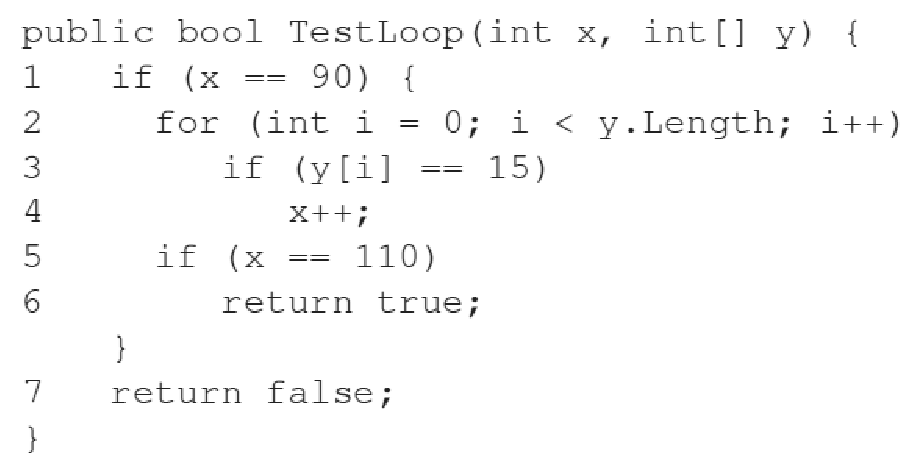
\includegraphics[scale=0.5]{fig/XiFitnessEPS.eps}
\caption{Figure 1. An example method under test.}
\end{figure}
\indent Random testing is one of the most commanly used technique for structural software testing since its easy implementation and the marginal overhead in choosing inputs. It simply generates the test input randomly and feed the input to the program under test. Even though the unbiased and effiecient nature of random testing, it will face difficulty to cover a certain statement or branch whose execution requires strict conditions on the input. For example, to cover the statement in line 6 of the example method in figure 1, the integer value of x needs to be exact 90, and the array of y contains more than 110 elements whose value are 15. This harsh condition on the input values makes it almost impossible to reach the statement in line 6.\\
\indent To address this issue faced by the random testing, dynamic symbolic execution(DSE) that systematically explores feasible paths of the program under test has been proposed recently. DSE executes the program for a given input, and performs collection of symbolic constraints on the inputs implied by predicate statements along the execution. The conjunction of all the conditions will be called path condition. DSE increases the code coverage by iteratively flipping the branch node of an already explored path and using constraint solver to generate test inputs based on the new path condition if it is satisfiable. For example, assuming the initial argument of x and y in the example method are 0 and \{0\}, respectively, the false branch of the line 1 statement, x!=90, is taken. Negating the branch will give the input value x=90 and y=\{0\} to cover the true branch of line 1. \\
\indent Even though DSE greatly improves the efficiency of achiving higher code coverage. It still faces multiple challenges in practical use. The covering of the true branch of line 5 needs exactly 20 executions of the true statement of line 3 inside the loop. By using DSE to hunt such a case, we would explore at least $2^{20}$ different execution paths before we can reach line 6 (using random searching strategy). This is in NP-Hard that renders the full coverage of the method almost impossible. 
\indent There are several other type of searching strategies besides random searching. DART ~\cite{dart}and CUTE ~\cite{cute} adoped the depth-first searching strategy and EXE ~\cite{exe}provide either depth-first search strategy and the mixture of best-first and depth-first strategy based on the code coverage heuristics. A generational search that explores only a very limited horizon are usd by SAGE~\cite{fuzz}.The drawbacks of all the searching strategies are biased nature that favor particular control flow points, e.g, the depth-first searching favors the final branches and the width-first searching strategy favors the first branches. None of these ways are capable of reaching target test stated in the example method efficientlly.\\
\indent To enhance the efficiency of DSE in achieving higher code coverage, the authors has proposed a novel way to guide DSE called fitnex, which is a searching strategy that uses state-dependent fitness values to guide path exploration. Through the fitness-guided path exploration, the full code coverage in cases like the example method under test will be more easily achieved. The procedure to use Fitnex strategy on the example method showed in figure 1 will be presented as follows:
\indent \textbf{Fitness computation for a path.} The fitness values are used to decide which branch's flipping would be more helpful in covering the target statement. Extracted from predicate of the conditions in executing test target, fitness functions are used to compute the fitness value, reflecting how close a path's execution is to the covering of the test target. The exploration then honors the fittest path which is the closest to the covering of the test target. The fitness function for the example method is $f(x)=|110-x|$. The smaller the fitness function value, the closer the path's execution is to cover the target. Considering the following 5 execution path,\\ 
\begin{center}
\begin{tabular}{|c|c|c|}\hline
Test & procedure & Path \\\hline
0 & TestLoop(0, new int[] {0}); & Path 0: 1F\\\hline
1 & TestLoop(90, new int[] {0}); & Path 1: 1T, 2T, 3F, 2F, 5F\\\hline
2 & TestLoop(90, new int[] {15}); &Path 2: 1T, 2T, 3T, 2F, 5F\\\hline
3 & TestLoop(90, new int[] {15, 0}); & Path 3: 1T, 2T, 3T, 2T, 3F, 2F, 5F\\\hline
4 & TestLoop(90, new int[] {15, 15});& Path 4: 1T, 2T, 3T, 2T, 3T, 2F, 5F\\\hline
\end{tabular}\\
Form 1. Several explored paths
\end{center}
Their fitness values for these paths are NA (for that the target test is not even reached), 20($|110 - 90|$), 19($|110 - 91|$), 19($|110 - 91|$), and 18(|110 - 92|) respectively. According to the proposed algorithm, the path 4 will be prefered since it the smallest value among all the paths which means that Path 4 is the closest path to the target test. Using symbolic value to compare fitness values may not to be a good idea since the comparison between symbolic values is quite expensive due to the invoking of constraint solver and the pairwise comparison is needed. Therefore, the concrete values are computed and compared. In general,  the predicate can be used to generate fitness functions to calculate how close a execution path to target test. The follwing form shows several instances, column 1 shows the predicate of the target test, column 2 shows the fitness function derived from it.\\
\begin{center}
\begin{tabular}{|c|c|}\hline
Predicate & Fitness function \\\hline
$F(a==b)$ & $|a-b|$ \\\hline
$F(a>b)$ & $(b-a)+k$ \\\hline
$F(a>=b)$ & $(b-a)$ \\\hline
$F(a<b)$ & $(a-b)+k$ \\\hline
$F(a<=b)$ & $(a-b)$ \\\hline
\end{tabular}\\
Form 2. Predicates and fitness function.
\end{center}
Besides the kind of predicates listed above, there is another category of target test that are guarded with boolean value rather than number value. In that case, deriving the fitness function will be much harder and no strategy has been proposed.
\indent\textbf{Fitness-gain computation for a branch.} Selecting branch node in a path to flip in order to approach the target test could be reduced to selecting a branch node that (1)has at least one new branch that has not been covered yet,(2)has the best potential to improve the fitness value of the current path. The fitness gain is defined as the decreasement of the fitness value before and after the flipping of a branch. The fitness gain could be used to prioritize the flipping of various branches. For example, the fitness-gain of flipping the branch in line 3 for path 1 is 1; The flipping of same branch in Path 3 will result in fitness-gain of same degree. Intuitively, not all the flipping will result in desirable fitness-gain. For example, the flip from true to false of line 3 in path 3 will cause the fitness-gain of -1.\\
\indent Each branch b in a path p is assigned a composite number $F(p)-FGain(b)$, whare $F(p)$ is the fitness value of the path p, and $FGain(b)$ is the fitness-gain of the flipping b in p. Then the priority of the flips all over the explored paths could be decided according to the composite value. Consider the previous four tests as a example, the smallest composite value comes at flipping the false branch in line 2 of the path 4 since the node has the least composite value 17. For several iterations, the strategy will eventually achieve the path whose fitness value is exactly 0, in another word, reach the target test.
